\chapter{Results and Discussion }

\section{Result of Comparison for various levels for Execution time}

Two files were given as input and one of these files is plagiarised and the other is source code i.e original.

\begin{itemize}
\item Level One Plagiarism Detection.

  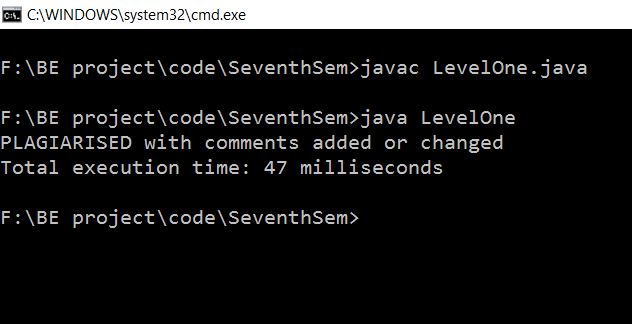
\includegraphics[width=.8\textwidth]{Level1}
  \label{fig:Level1}\\
  The plagiarised has comments and extra whitespace added.The program correctly identifies the that the file has been plagiarised.
   

\item Level Three Plagiarism Detection.

  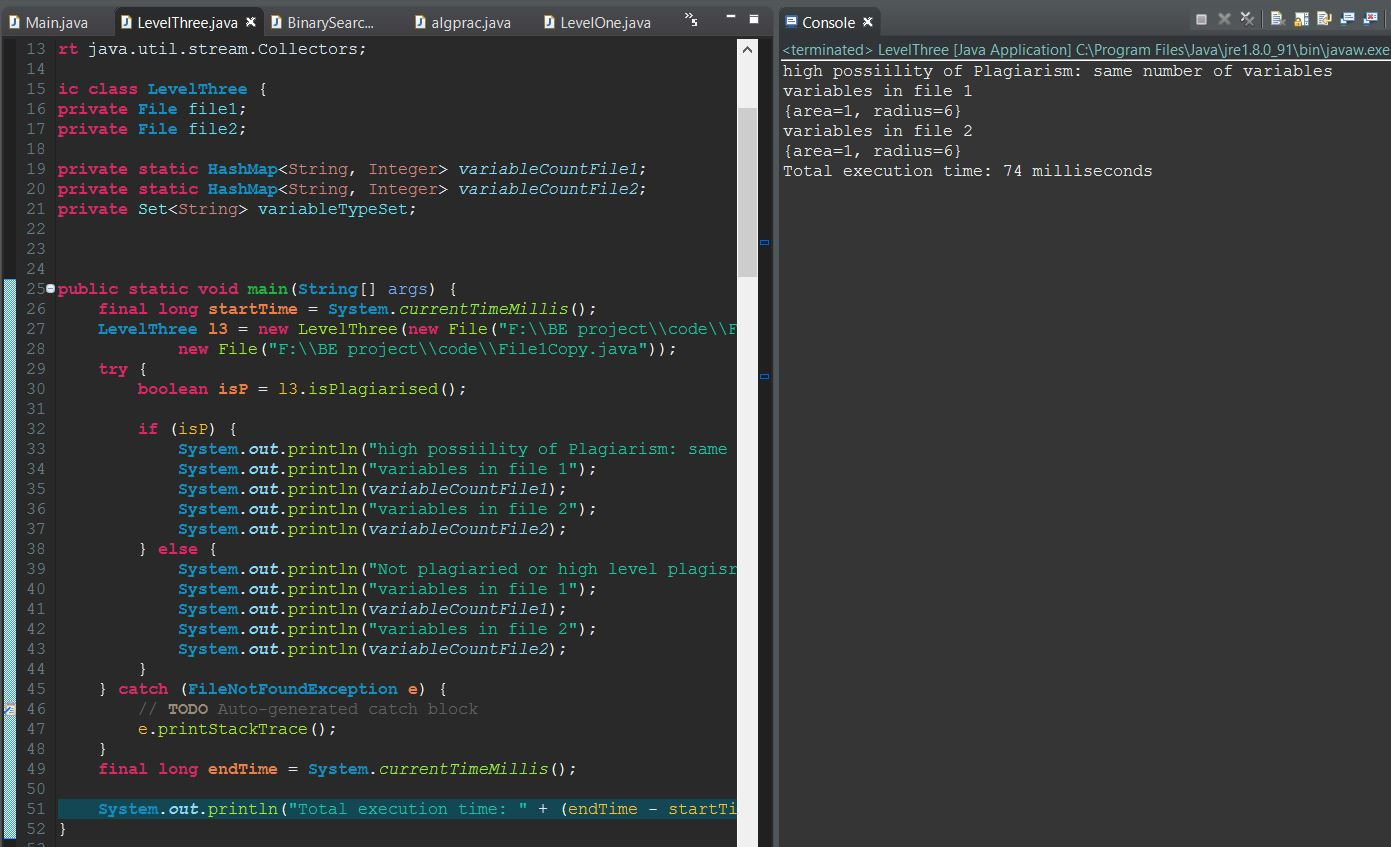
\includegraphics[width=.8\textwidth]{Level3}
  \label{fig:Level3}\\
  The plagiarised has changed the names of the variables and shifted their positions around the file.The program correctly identifies the that the file has been plagiarised.
  
\item Result from JPlag.

  \includegraphics[width=.8\textwidth]{JPlag}
  \label{fig:JPlag}\\
  These two files were given as an input to the popular plagiarism detction software tool called JPlag and the results shown by this tool matched the result given by our program.
   
  
\item Result from MOSS.



  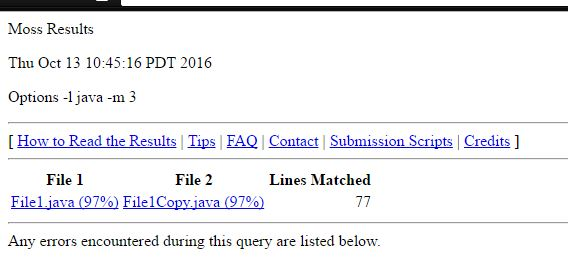
\includegraphics[width=.8\textwidth]{MOSS}
  \label{fig:MOSS}\\
  
These two files were given as an input to the popular plagiarism detction software tool called MOSS and the results shown by this tool matched the result given by our program.

\end{itemize}
